%========================================
% LESSON CONTENT: Propiedades de los Números Reales y Exponentes
%========================================

\lesson{Propiedades de los Números Reales y Exponentes}

\subsectiontitle{Clasificación de los Números}

\begin{definition}
La jerarquía de los números reales se estructura de la siguiente manera:
$$\text{Números Reales} \begin{cases}
\text{Números Racionales} \begin{cases}
\text{Enteros} \begin{cases}
\text{Enteros Negativos} \\
0 \\
\text{Enteros Positivos}
\end{cases}
\end{cases} \\
\text{Números Irracionales}
\end{cases}$$
\end{definition}

\subsectiontitle{Números Enteros}

\begin{definition}
El conjunto de los \textbf{números enteros} consiste de la unión del conjunto de los números enteros positivos (o números naturales), el conjunto de los enteros negativos y el cero.
$$\mathbb{Z} = \{\ldots, -3, -2, -1, 0, 1, 2, 3, \ldots\}$$
\end{definition}

\textbf{Características:}
\begin{itemize}
\item Incluye todos los números naturales: $1, 2, 3, 4, \ldots$
\item Incluye el cero: $0$
\item Incluye todos los números negativos: $-1, -2, -3, \ldots$
\item No incluye fracciones ni decimales
\end{itemize}

\subsectiontitle{Números Racionales}

\begin{definition}
El conjunto de los \textbf{números racionales} consiste de todos los números que pueden expresarse como la \textbf{razón} de dos números enteros.
$$r = \frac{m}{n}, \quad m, n \text{ enteros}, \quad n \neq 0$$
\end{definition}

\textbf{Características importantes:}
\begin{itemize}
\item Todo entero es racional: $5 = \frac{5}{1}$
\item Las fracciones son racionales: $\frac{3}{4}, \frac{-7}{2}$
\item Los decimales finitos son racionales: $0.25 = \frac{1}{4}$
\item Los decimales periódicos son racionales
\end{itemize}

La notación $\mathbb{Q}$ proviene de ``quotient'' (cociente en inglés).

\subsectiontitle{Números Irracionales}

\begin{definition}
El conjunto de los \textbf{números irracionales} consiste de todos los números que \textbf{NO} pueden expresarse como el cociente de dos números enteros.
\end{definition}

\begin{example}
Ejemplos de números irracionales:
\begin{itemize}
\item $\sqrt{3}$ (raíz cuadrada de 3)
\item $\sqrt{5}$ (raíz cuadrada de 5)
\item $\sqrt[3]{2}$ (raíz cúbica de 2)
\item $\pi$ (pi, aproximadamente 3.14159...)
\end{itemize}

Características:
\begin{itemize}
\item Su representación decimal es infinita y no periódica
\item No se pueden escribir como fracción de enteros
\item Son fundamentales en geometría y cálculo
\end{itemize}
\end{example}

\subsectiontitle{Números Reales}

\begin{definition}
El conjunto de los \textbf{números reales} consiste de la unión del conjunto de los números racionales y el conjunto de los números irracionales.
$$\mathbb{R} = \mathbb{Q} \cup \text{Irracionales}$$
\end{definition}

\textbf{Propiedad importante:} Todo número real tiene una \textbf{representación decimal} única.

\subsectiontitle{Representación Decimal}

\textbf{Para Números Racionales:} Si el número es racional, su parte decimal correspondiente \textbf{se repite}.

\begin{example}
$$\frac{1}{3} = 0.33333\ldots = 0.\overline{3}$$
$$\frac{5}{7} = 0.714285714\ldots = 0.\overline{714285}$$
\end{example}

\textbf{Para Números Irracionales:} Si el número es irracional, su parte decimal correspondiente \textbf{NO se repite}.

\begin{example}
$$\sqrt{5} = 2.236067978\ldots$$
$$\pi = 3.141592654\ldots$$
\end{example}

\subsectiontitle{Representación Gráfica: Recta Numérica}

Podemos representar a los números reales de forma gráfica, mediante puntos colocados en una recta numérica.

% Number line visualization
\begin{center}
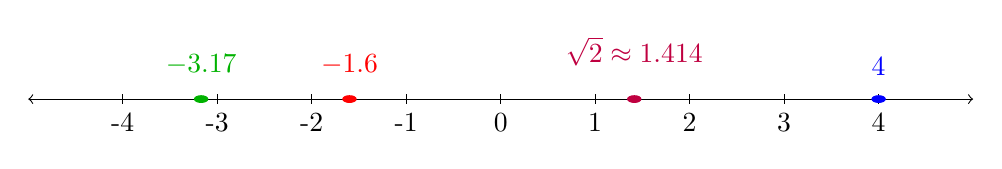
\begin{tikzpicture}[scale=0.6, xscale=2]
    % Number line
    \draw[<->] (-5,0) -- (5,0);
    \foreach \x in {-4,-3,-2,-1,0,1,2,3,4}
        \draw (\x,0.1) -- (\x,-0.1) node[below] {\x};
    
    % Special points
    \filldraw[red] (-1.6,0) circle (2pt);
    \node[red, above] at (-1.6,0.3) {$-1.6$};
    
    \filldraw[blue] (4,0) circle (2pt);
    \node[blue, above] at (4,0.3) {$4$};
    
    % Additional examples
    \filldraw[green!70!black] (-3.17,0) circle (2pt);
    \node[green!70!black, above] at (-3.17,0.3) {$-3.17$};
    
    \filldraw[purple] (1.414,0) circle (2pt);
    \node[purple, above] at (1.414,0.5) {$\sqrt{2} \approx 1.414$};
\end{tikzpicture}
\end{center}

\subsectiontitle{Propiedades de los Números Reales}

Las propiedades fundamentales de los números reales forman la base del álgebra. Estas se organizan en categorías:

% Property visualization flowchart
\begin{center}
\begin{tikzpicture}[
    property/.style={rectangle, draw=blue!60, fill=blue!5, thick, minimum height=1cm, text width=3.5cm, text centered},
    example/.style={rectangle, draw=green!60, fill=green!5, text width=4cm, text centered},
    arrow/.style={-{Stealth[length=3mm]}, thick}
]
    % Commutative Properties
    \node[property] (comm) at (0,0) {\textbf{Propiedades Conmutativas}};
    \node[example] (comm_add) at (-3,-1.8) {$a + b = b + a$\\$2 + 3 = 3 + 2$};
    \node[example] (comm_mult) at (3,-1.8) {$ab = ba$\\$4 \cdot 2 = 2 \cdot 4$};
    
    % Associative Properties  
    \node[property] (assoc) at (0,-3.5) {\textbf{Propiedades Asociativas}};
    \node[example] (assoc_add) at (-3,-5.3) {$(a+b)+c = a+(b+c)$\\$(2+3)+7 = 2+(3+7)$};
    \node[example] (assoc_mult) at (3,-5.3) {$(ab)c = a(bc)$\\$(3 \cdot 7) \cdot 5 = 3 \cdot (7 \cdot 5)$};
    
    % Distributive Property
    \node[property] (dist) at (0,-7) {\textbf{Propiedad Distributiva}};
    \node[example] (dist_ex) at (0,-8.8) {$a(b+c) = ab + ac$\\$4(2+6) = 4 \cdot 2 + 4 \cdot 6$};
    
    % Arrows
    \draw[arrow] (comm) -- (comm_add);
    \draw[arrow] (comm) -- (comm_mult);
    \draw[arrow] (assoc) -- (assoc_add);
    \draw[arrow] (assoc) -- (assoc_mult);
    \draw[arrow] (dist) -- (dist_ex);
\end{tikzpicture}
\end{center}

\begin{definition}
\textbf{Propiedades Conmutativas:} El orden de los términos no afecta el resultado.
\begin{itemize}
\item \textbf{Suma:} $a + b = b + a$
\item \textbf{Multiplicación:} $ab = ba$
\end{itemize}
\end{definition}

\begin{definition}
\textbf{Propiedades Asociativas:} La agrupación de los términos no afecta el resultado.
\begin{itemize}
\item \textbf{Suma:} $(a + b) + c = a + (b + c)$
\item \textbf{Multiplicación:} $(ab)c = a(bc)$
\end{itemize}
\end{definition}

\begin{definition}
\textbf{Propiedad Distributiva:} La multiplicación se distribuye sobre la suma.
$$a(b + c) = ab + ac$$
\end{definition}

\subsectiontitle{Elementos Neutros}

\begin{definition}
\textbf{Neutro Aditivo:} El número $0$ se le llama el \textbf{neutro aditivo}. Cumple la siguiente propiedad para cualquier número real $a$:
$$a + 0 = a$$
\textbf{Explicación:} Sumar cero a cualquier número no cambia el valor del número.
\end{definition}

\begin{definition}
\textbf{Neutro Multiplicativo:} El número $1$ se le llama el \textbf{neutro multiplicativo}. Cumple la siguiente propiedad para cualquier número real $a$:
$$a \cdot 1 = a$$
\textbf{Explicación:} Multiplicar cualquier número por uno no cambia el valor del número.
\end{definition}

\subsectiontitle{Elementos Inversos}

\begin{definition}
\textbf{Negativo de un Número Real (Inverso Aditivo):} Todo número real $a$ tiene un \textbf{negativo} (o inverso aditivo), denotado $-a$, que satisface:
$$a + (-a) = 0$$
\end{definition}

\begin{example}
$-3$, se lee ``negativo 3'' o ``el opuesto de 3''.
$$3 + (-3) = 0$$
\end{example}

\begin{definition}
\textbf{Inverso Multiplicativo:} Cualquier número real $a$ (con $a \neq 0$) tiene un \textbf{inverso multiplicativo}, denotado $\frac{1}{a}$, que cumple:
$$a \cdot \left(\frac{1}{a}\right) = 1, \quad a \neq 0$$
\end{definition}

\begin{example}
\begin{itemize}
\item El inverso multiplicativo de $5$ es $\frac{1}{5}$
\item El inverso multiplicativo de $\frac{2}{3}$ es $\frac{3}{2}$
\end{itemize}
\end{example}

\subsectiontitle{Operaciones Inversas}

\begin{definition}
\textbf{Resta: Operación Inversa de la Suma}
La resta es la operación inversa de la suma. Toda resta se puede expresar como una suma:
$$a - b = a + (-b)$$
\end{definition}

\begin{example}
$7 - 3 = 7 + (-3) = 4$
\end{example}

\begin{definition}
\textbf{División: Operación Inversa de la Multiplicación}
La división es la operación inversa de la multiplicación. Para dividir por un número, multiplicamos por el inverso de dicho número:
$$a \div b = a \cdot \frac{1}{b} = \frac{a}{b}, \quad b \neq 0$$
\end{definition}

\begin{example}
$12 \div 4 = 12 \cdot \frac{1}{4} = 3$
\end{example}

\subsectiontitle{Exponentes}

\begin{definition}
Sea $a$ cualquier número real, $n$ un entero positivo. La \textbf{n-ésima potencia} de $a$, se expresa:
$$a^n = \underbrace{a \cdot a \cdot a \cdots a}_{n \text{ factores}}$$
\end{definition}

\begin{example}
\begin{itemize}
\item $2^3 = 2 \cdot 2 \cdot 2 = 8$
\item $5^2 = 5 \cdot 5 = 25$
\item $(-3)^4 = (-3) \cdot (-3) \cdot (-3) \cdot (-3) = 81$
\end{itemize}

\textbf{Terminología:}
\begin{itemize}
\item En $a^n$: $a$ se llama la \textbf{base}
\item En $a^n$: $n$ se llama el \textbf{exponente}
\end{itemize}
\end{example}

\subsectiontitle{Orden de Operaciones}

Cuando realizamos operaciones aritméticas, debemos seguir el orden apropiado:

% PEMDSR visual memory aid
\begin{center}
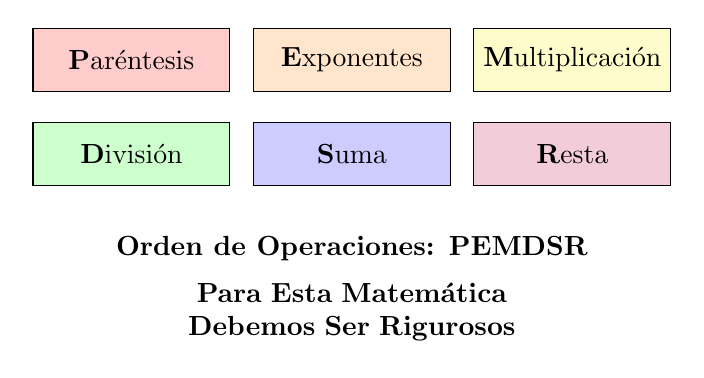
\begin{tikzpicture}[scale=0.8]
    \node[draw, fill=red!20, minimum width=2.5cm, minimum height=0.8cm] at (0,0) {\textbf{P}aréntesis};
    \node[draw, fill=orange!20, minimum width=2.5cm, minimum height=0.8cm] at (3.5,0) {\textbf{E}xponentes};
    \node[draw, fill=yellow!20, minimum width=2.5cm, minimum height=0.8cm] at (7,0) {\textbf{M}ultiplicación};
    \node[draw, fill=green!20, minimum width=2.5cm, minimum height=0.8cm] at (0,-1.5) {\textbf{D}ivisión};
    \node[draw, fill=blue!20, minimum width=2.5cm, minimum height=0.8cm] at (3.5,-1.5) {\textbf{S}uma};
    \node[draw, fill=purple!20, minimum width=2.5cm, minimum height=0.8cm] at (7,-1.5) {\textbf{R}esta};
    
    \node at (3.5,-3) {\textbf{Orden de Operaciones: PEMDSR}};
    
    % Mnemonic aid
    \node[text width=8cm, text centered] at (3.5,-4) {
        \textbf{Para Esta Matemática Debemos Ser Rigurosos}
    };
\end{tikzpicture}
\end{center}

\begin{example}
Evaluar: $3 + 4 \times 2^2$

\textbf{Paso a paso:}
\begin{align}
3 + 4 \times 2^2 &= 3 + 4 \times 4 && \text{(Exponentes primero)}\\
&= 3 + 16 && \text{(Multiplicación)}\\
&= 19 && \text{(Suma)}
\end{align}
\end{example}

\subsectiontitle{Fracciones}

\begin{definition}
En la expresión $\frac{a}{b}$ donde $b \neq 0$, llamamos:
\begin{itemize}
\item $a$ : \textbf{Numerador}
\item $b$ : \textbf{Denominador}
\end{itemize}
\end{definition}

\textbf{Propiedades fundamentales de las fracciones:}

\begin{theorem}
\textbf{Multiplicación de fracciones:}
$$\frac{a}{b} \cdot \frac{c}{d} = \frac{ac}{bd}$$
Para multiplicar fracciones, se multiplican los numeradores y los denominadores entre sí.
\end{theorem}

\begin{example}
$\frac{3}{5} \cdot \frac{2}{7} = \frac{3 \cdot 2}{5 \cdot 7} = \frac{6}{35}$
\end{example}

\begin{theorem}
\textbf{División de fracciones:}
$$\frac{a}{b} \div \frac{c}{d} = \frac{a}{b} \cdot \frac{d}{c}$$
Para dividir fracciones, se invierte el divisor y se multiplica.
\end{theorem}

\begin{example}
$\frac{3}{5} \div \frac{2}{7} = \frac{3}{5} \cdot \frac{7}{2} = \frac{21}{10}$
\end{example}

\begin{theorem}
\textbf{Suma de fracciones con igual denominador:}
$$\frac{a}{c} + \frac{b}{c} = \frac{a + b}{c}$$
\end{theorem}

\begin{example}
$\frac{1}{5} + \frac{2}{5} = \frac{1 + 2}{5} = \frac{3}{5}$
\end{example}

\begin{theorem}
\textbf{Suma de fracciones con diferentes denominadores:}
$$\frac{a}{b} + \frac{c}{d} = \frac{ad + bc}{bd}$$
\end{theorem}

\begin{example}
$\frac{2}{5} + \frac{3}{7} = \frac{2(7) + 3(5)}{5(7)} = \frac{14 + 15}{35} = \frac{29}{35}$
\end{example}